\documentclass[a4paper,12pt,twoside]{article}
\usepackage{fontspec}
\setmainfont{Times New Roman}
\usepackage[a4paper,left=25mm,right=25mm,bottom=25mm,top=25mm]{geometry}
\usepackage{hyperref}
\usepackage{url}
\usepackage{float}
\usepackage{subcaption}
\usepackage{amsmath}
\usepackage{graphicx}
\usepackage{color}
\usepackage[style=numeric]{biblatex}
\addbibresource{references.bib}
\usepackage{multirow}
\usepackage{makecell}
% \usepackage{xcolor} 
% \pagecolor[rgb]{0.12,0.12,0.12} 
% \color[rgb]{1,1,1}

\begin{document}

\title{Completely Contactless and Online Finger Knuckle Identification}

\setlength{\parindent}{0em}
\setlength{\parskip}{0.5em}
\author{Zhenyu ZHOU}
\date{\today}
\maketitle

\section{Whole Image Translated and Rotated Triplet Loss Function}

Because our neural networks were trained using the architecture of triplet network \cite{schroff2015facenet}, we used translated and rotated triplet loss function (TRTLoss) as loss function to update convolutional kernel of our models. When we match two finger knuckles in the contactless scenario, they will not only translate but also will rotate with local deformable transformation. For solving it, we add rotation based on translation to compose a more robust transformation. As for the TRTLoss function, we rotate feature maps while translate feature maps based on the Soft-Shifted Triplet Loss Function \cite{liu2020contactless}.

\vspace{10pt}

In generally, the TRTLoss is still a variant of triple loss, so that the TRTLoss can be written as a format of triple loss function as the Equation \ref{Tripletloss}. As for the $N$, it means the number of triplet during training iteration, and $F(I^{a})$ is the output feature map of input anchor image $I^a$ through neural network. The hard margin parameter $m$ can determine the distance between different class cluster by pushing them away.
\begin{equation}
	\begin{aligned}
		TRTLoss = \frac{1}{N}\sum_{i}^{N}[L(F(I_{i}^{a}),F(I_{i}^{p}))-L(F(I_{i}^{a}),F(I_{i}^{n})) + m]_{+}
	\end{aligned}
	\label{Tripletloss}
\end{equation}

We add translation and rotation transformation to deal with local deformable of finger knuckle. In order to adapt to tasks with different degrees of deformation, and balance performance and speed, we set translation and rotation ranges as a hyperparameter. The $L(F_1, F_2)$ will get the minimal distance of two feature maps $D_{w,h,\theta}(F_1, F_2)$ after translation and rotation in the range $-W{\leq}w{\leq}W, -H{\leq}h{\leq}H, {-\Theta}{\leq}\theta{\leq}{\Theta}$. Meanwhile, the distance $D_{w,h,\theta}(F_1, F_2)$ calculates the pixel-wise MSE value when feature map is translated $w$ pixel along x-axis and $h$ pixel along y-axis and rotated $\theta$ angle in the Equation \ref{Distance}.
\begin{equation}
	\begin{aligned}
		L(F_1, F_2) = \mathop{min}\limits_{-W{\leq}w{\leq}W, -H{\leq}h{\leq}H, {-\Theta}{\leq}\theta{\leq}{\Theta}}{D_{w,h,\theta}(F_1, F_2)}
	\end{aligned}
\end{equation}
\begin{equation}
	\begin{aligned}
		D_{w,h,\theta}(F_1, F_2) = \frac{1}{|C_{w,h,\theta}|}\sum_{(x,y){\in}C_{w,h,\theta}}(F_1^{(w,h,\theta)}[x,y] - F_2[x,y])^2
	\end{aligned}
	\label{Distance}
\end{equation}

In terms of $C_{w,h,\theta}$, it represents the common region between two feature maps after one feature map shifted along x-axis with w, shifted along y-axis with h, and rotated with $\theta$. As for the $(F_a, F_p)$ pair, we can assume when the $F_a$ is rotated angle of $\theta_{ap}$ and shifted with ($w_{ap}$, $h_{ap}$) pixels can get the minimal $D_{w_{ap},h_{ap},\theta_{ap}}(F_a, F_p)$, then $L(F_a, F_p) = D_{w_{ap},h_{ap},\theta_{ap}}(F_a, F_p)$. Meanwhile, with the $(w_{an}, h_{an}, \theta_{an})$, the $(F_a, F_n)$ pair can get the minimal $D_{w_{an},h_{an},\theta_{an}}(F_a, F_m)$.
\begin{equation}
	\begin{aligned}
		\frac{\partial{Loss}}{\partial{F_i^p}}=
		\begin{cases}
			0, if (x,y) \notin {C_{w_{ap}, h_{ap}, \theta_{ap}}}{\ }or{\ }Loss = 0 \\
			\frac{-2(F_i^a[[x_{w_{ap}}, y_{h_{ap}}]*M(\theta_{ap})]-F_i^p[x,y])}{N|C_{w_{ap},h_{ap},\theta_{ap}}|},otherwise
		\end{cases}
	\end{aligned}
\end{equation}
The $M(\theta_{ap})$ is the rotation matrix.

\begin{equation}
	\begin{aligned}
		\frac{\partial{Loss}}{\partial{F_i^n}}=
		\begin{cases}
			0, if (x,y) \notin {C_{w_{an}, h_{an}, \theta_{an}}}{\ }or{\ }Loss = 0 \\
			\frac{-2(F_i^a[[x_{w_{an}}, y_{h_{an}}]*M(\theta_{an})]-F_i^n[x,y])}{N|C_{w_{an},h_{an},a_{an}}|}, otherwise
		\end{cases}
	\end{aligned}
\end{equation}

As for the $F_i^a[x,y]$ derivation, because we shift and rotate the anchor in the above formula, we can inversely shift and rotate the positive and negative input feature.
\begin{equation}
	\begin{aligned}
		\frac{\partial{Loss}}{\partial{F_i^a[x,y]}} = -\frac{\partial{Loss}}{\partial{F_i^p[[x-w_{ap}, y-h_{ap}]*M(-\theta_{ap})]}} + \\
		 \frac{\partial{Loss}}{\partial{F_i^n[[x-w_{an}, y-h_{an}]*M(-\theta_{an})]}}
	\end{aligned}
\end{equation}
\section{Experiments and Results}
In this part, We will compare Translation and Rotation Triplet Loss (TRTL) and Shift Translation Triplet Loss \cite{liu2020contactless} performance on different finger knuckle dataset. Meanwhile, we will also compare with the state-of-the-art FKNet and EfficientNetV2. All the experiment will use the finger knuckle segmented by YOLOv5-CSL as training set and testing set. In the Online Contactless Finger Knuckle Identification section, we will compare the impact of the finger knuckle segmented by YOLOV5 and the finger knuckle provided by these databases on the performance. 

As for the DeConvRFNet, we just change the RFNet \cite{liu2020contactless} convolution layer with deformable convolution layer. Then as for DeConvRFNet and RFNet model, we pretrained on the Finger Knuckle V1 Database \cite{fingerknuckledbv1.0}.EfficientNetV2-S is the original classification model, we keep the same architecture and just change the FC layer of the head part with convolution layer for fitting TRTL and STTL to compose EfficientNetV2-S-STTL and EfficientNetV2-S-TRTL model. When trained these EfficientNetV2-S model, we use the pretrained weight on the ImageNet21K. As for the FKNet, we use the pretrained ResNet-50 weights.

Because the EfficientNetV2-S and FKNet is a classification model, I calculate MSE of two feature vectors of last layer of model as matching score. And as for the input data, I follow the same method of FKNet, each image will rotate from $-10^{\circ}$ to $10^{\circ}$ to increase the amount of training data.

\subsection{Model Complexity Analysis}
.........
\input{FK-Identification/fingerknucklev3.tex}
\input{FK-Identification/indexfingerofhd.tex}
\input{FK-Identification/2dof3dfingerknuckle.tex}
\subsection{Cross-Database Experiments}

I firstly pre-trained my models on the Finger Knuckle V1 Database, and then fine-tuned models on the Finger Knuckle V3 Database (with deformable). I use these kind training method, and use these models to test performance on the Index Finger Knuckle of Hand Dorsal Image and Tsinghua Finger Knuckle Database as a cross database experiment. The label in the finger curve, the content in parentheses indicates the training samples. Such as RFN-WS(1-104), it uses 1-104 subjects of Finger Knuckle V3 Database to train models. Updated ROC Curve and CMC Curve with RFNet, EfficientNet and DeConvRFNet. For the ROC curve, I add EfficientNetV2-S model performance.

\subsubsection{Index Finger Knuckle of Hand Dorsal Image}

\begin{figure}[H]
	\centering
	\begin{subfigure}[b]{0.45\linewidth}
		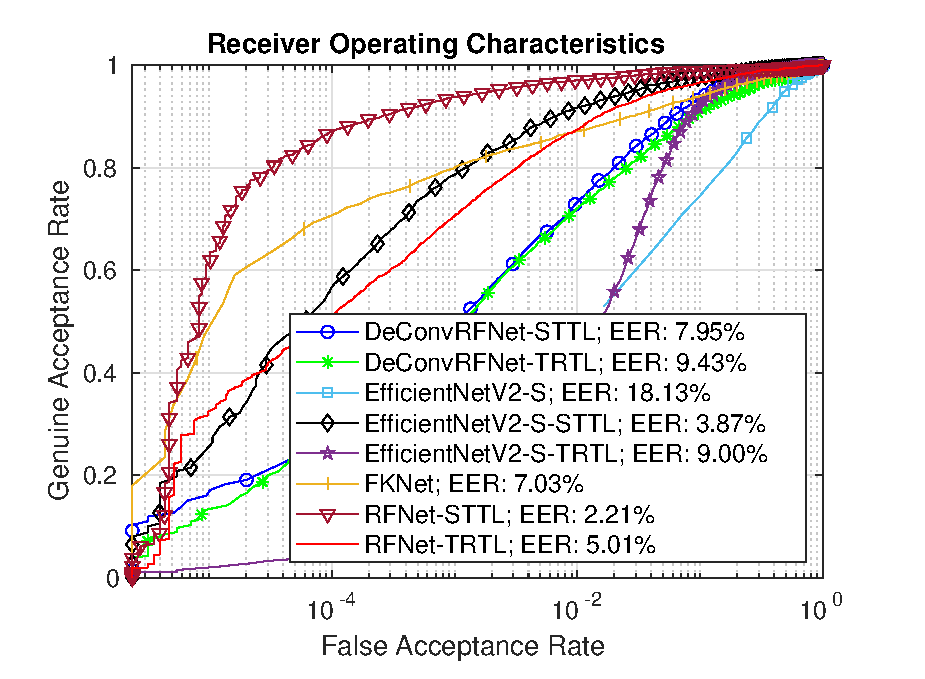
\includegraphics[width=\linewidth]{Figures/crosshd-roc_compare_new.eps}
	\end{subfigure}
    \begin{subfigure}[b]{0.45\linewidth}
		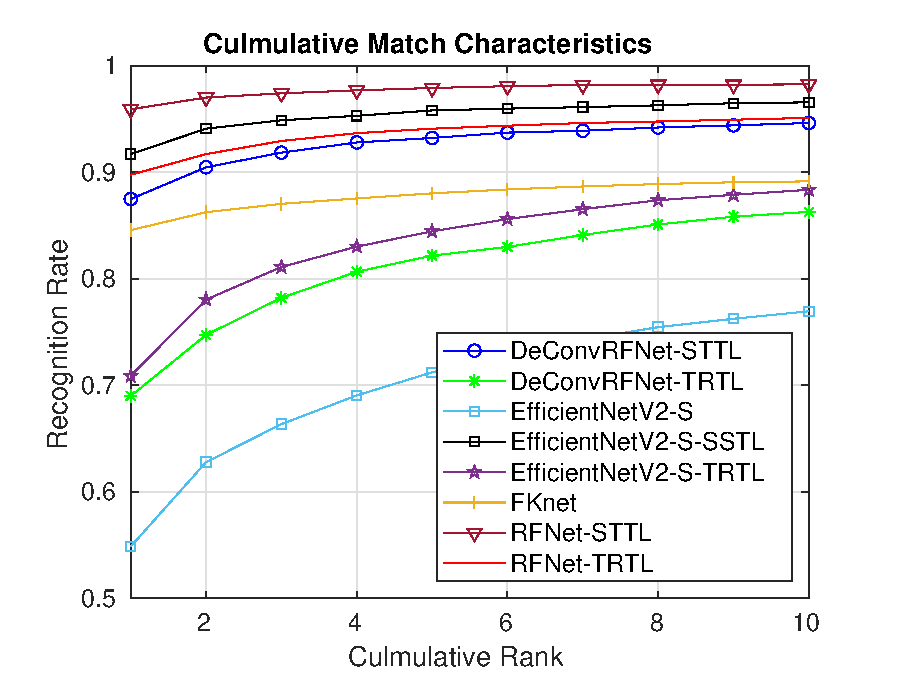
\includegraphics[width=\linewidth]{Figures/crosshd-cmc_compare_new.eps}
	\end{subfigure}
\end{figure}

The database totally has 712 subjects, and each subject has 5 samples. Therefore, it will have $712*5$ genuine matching scores and $712*711*5$ imposter matching scores. From the cure, the performance of RFN-WS and RFN-WRS is similar, and the RFN-WS is slightly better than RFN-WRS while using the same training samples. Updated ROC Curve and CMC Curve with RFNet, EfficientNet and DeConvRFNet. For the ROC curve, I add EfficientNetV2-S model performance.

\subsubsection{Middle Finger Knuckle of Hand Dorsal Image}
\begin{figure}[H]
	\centering
	\begin{subfigure}[b]{0.45\linewidth}
		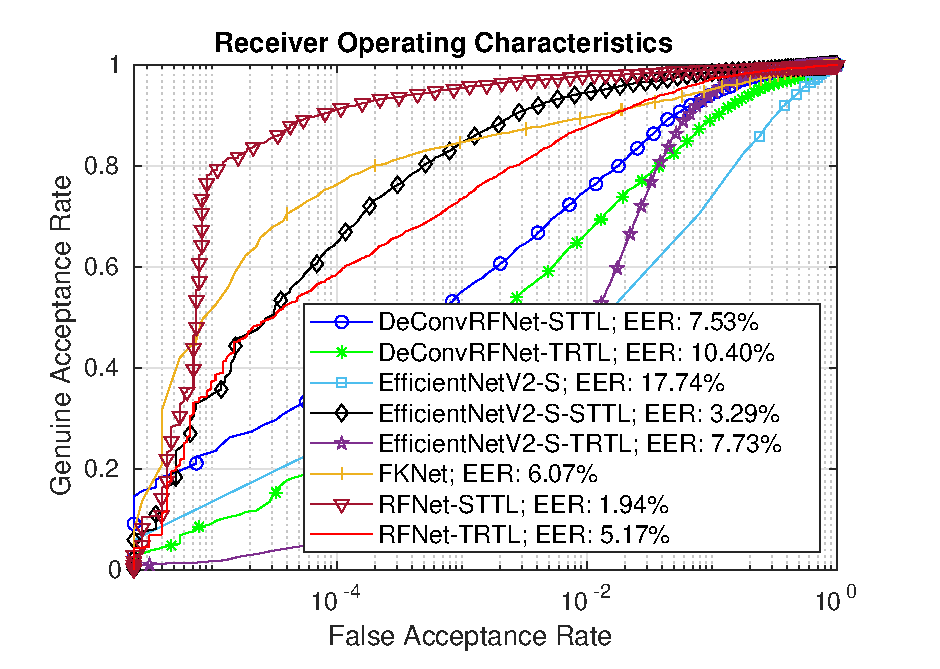
\includegraphics[width=\linewidth]{Figures/crosshd-middle-roc_compare_new.eps}
	\end{subfigure}
    \begin{subfigure}[b]{0.45\linewidth}
		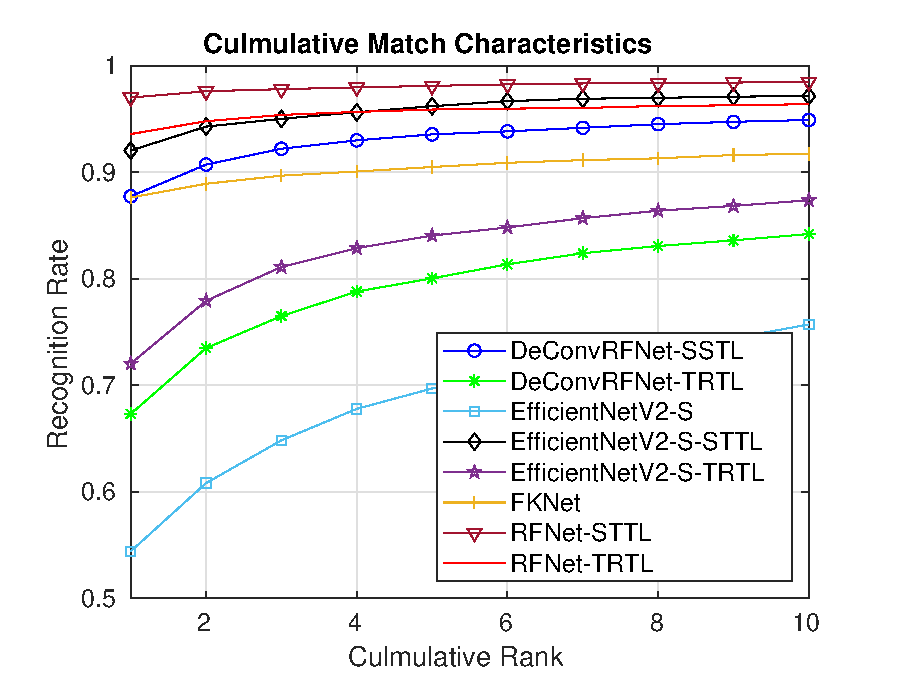
\includegraphics[width=\linewidth]{Figures/crosshd-middle-cmc_compare_new.eps}
	\end{subfigure}
\end{figure}


\subsubsection{Tsinghua Finger Knuckle Database}
\begin{figure}[H]
	\centering
	\begin{subfigure}[b]{0.45\linewidth}
		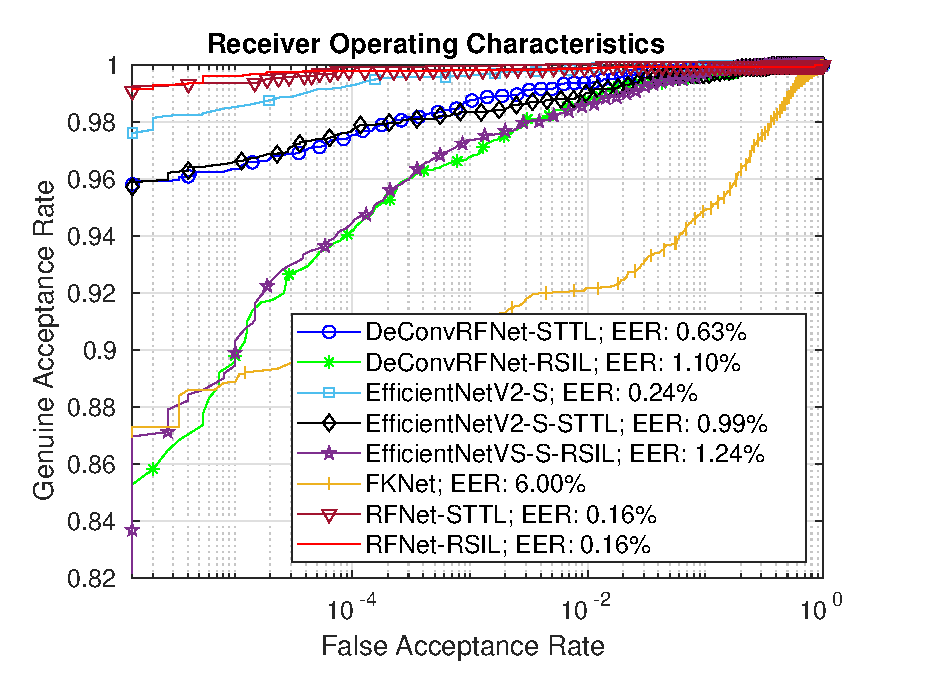
\includegraphics[width=\linewidth]{Figures/crossthu-roc_compare_new.eps}
	\end{subfigure}
    \begin{subfigure}[b]{0.45\linewidth}
		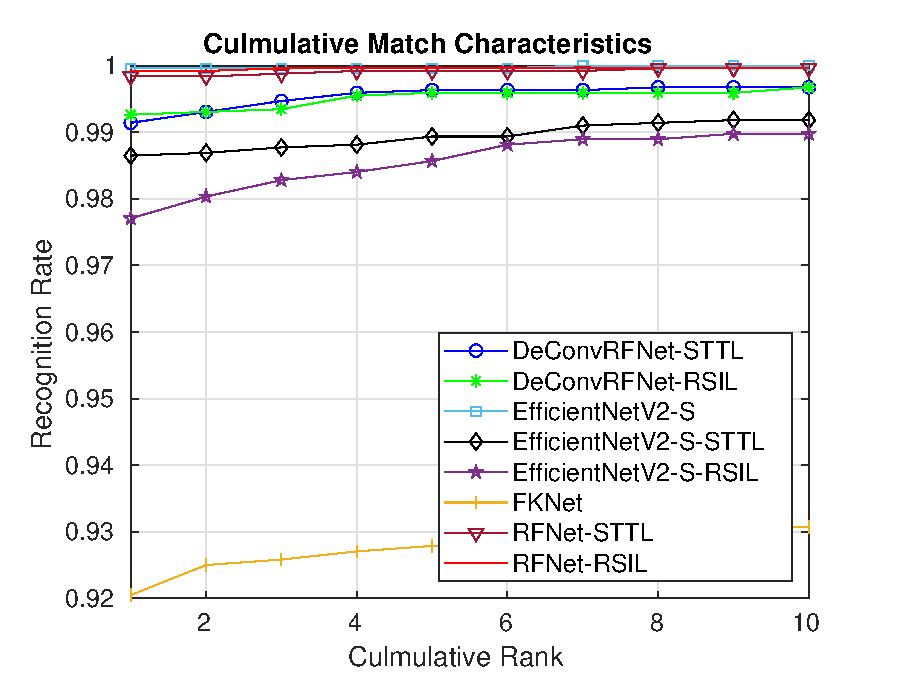
\includegraphics[width=\linewidth]{Figures/crossthu-cmc_compare_new.eps}
	\end{subfigure}
\end{figure}

The database has 610 subjects, and each subject can offer 4 samples. Then as the cross database experiment, it will have $610*4$ genuine matching scores and $610*609*4$ imposter matching scores. In this database, all models can get very high matching performance from the table and figure.

\subsection{Discussion}
From these experiment results, we can see that EfficientV2-S model is better than FKNet in some dataset. Becuase EfficientNetV2 model use MBConv as a block unit for replacing residual block. As for MBConv block, it use depthwise convolutions to decrease training weights and use Squeeze-Excited block as channel tranfomer. Meanwhile, the depth of EfficientNetV2-S is deeper than the FKNet.

There is another conclusion is that TRTL generalization ablity is lower thant STTL loss from the cross database experiment. But in the within database experiment, these model with TRTL loss is better thant STTL loss.

..............

\subsection{3D Finger Knuckle Images Database}

Because the RFNet with TRTL and STTL can get the best performance on the within database experiment and cross database experiment, 

I have used the matlab code that offered by the FKNet to generate the 3D finger knuckle images for getting the depth information. But it is different that the input image size. The FKNet will resize the original image size $148*212$ to $70*100$ as the testing dataset, and crop from the $70*100$ to $48*80$ as the training dataset. As for RFNet, I just use the original image as the input data. Then the experiment protocol will generate $190*6$ genuine matching scores, and $190*189*6$ imposter matching scores. From the experiment result, we can get that the RFNet is the best model for the 3D Finger Knuckle Database.

\begin{figure}[H]
    \centering
    \begin{subfigure}[b]{0.45\linewidth}
        \includegraphics[width=\linewidth]{Figures/3dod3d-roc_compare_new.eps}
    \end{subfigure}
    \begin{subfigure}[b]{0.45\linewidth}
        \includegraphics[width=\linewidth]{Figures/3dod3d-cmc_compare_new.eps}
    \end{subfigure}
\end{figure}


\subsection{Discussion}
From these experiment results, we can see that EfficientV2-S model is better than FKNet in some dataset. Because EfficientNetV2 model use MBConv as a block unit for replacing residual block. As for MBConv block, it uses depth-wise convolutions to decrease training weights and use Squeeze-Excited block as channel transformer. Meanwhile, the depth of EfficientNetV2-S is deeper than the FKNet.

There is another conclusion is that TRTL generalization ability is lower than STTL loss from the cross database experiment. But in the within database experiment, these model with TRTL loss is better than STTL loss.

..............
\input{FK-Identification/yolov5segmentvsdataoffter.tex}
\section{Online Contactless Finger Knuckle Identification}

With RSIL loss, the RFNet \cite{liu2020contactless} can outperform state-of-the-art methods. In the previous section, we have estimated its verification and identification performance on different public finger knuckle database, including within-db and cross-db experiments. As for a completely contactless and online finger knuckle identification, the finger knuckle detector is a very important module for automatically detect and segment finger knuckle region. However, as for traditional segmentation algorithm, they cannot correctly segment the finger knuckles in the presence of complex background interference, multiple finger knuckles in the same field of view, obscured finger knuckles or bent finger knuckles.
Meanwhile, as for neural network, the current based on YOLO \cite{redmon2016you}, \cite{redmon2017yolo9000}, \cite{redmon2018yolov3}, \cite{bochkovskiy2020yolov4}, \cite{YOLOv5} and R-CNN \cite{girshick2014rich}, \cite{girshick2015fast}, \cite{ren2015faster}, \cite{he2017mask} series object detection and segmentation approaches cannot simultaneously obtain the angle of finger knuckle and the segmentation with high precision. Especially, the angle of the finger knuckle is a vital factor for identification. If we can get the angle of finger knuckle, we can use angle information to align two feature maps for increasing matching accuracy and efficiency. For solving above problems, we propose rotated bounding box detection based on YOLOv5 model for segmenting and getting angle information.

\subsection{Contactless Finger Knuckle Detection}
\subsubsection{ Oriented Bounding Box Based on YOLOv5}
In order to solve the problem of finger knuckle detection in the real world, we choose to use YOLOv5 model because the YOLO series is famous for its fast detection speed and high accuracy. Especially, the YOLOv5's \cite{YOLOv5} speed can meet our online detection requirements.

\noindent\textbf{Oriented Bounding Box}

\begin{figure}[ht!]
	\centering
	\begin{subfigure}[b]{0.45\linewidth}
		\centering
		\includegraphics[width=0.6\linewidth]{Figures/five-parameter-definition.png}
		\caption{Five-parameter definition with $180^{\circ}$ angular range.}
	\end{subfigure}
	\begin{subfigure}[b]{0.45\linewidth}
		\centering
		\includegraphics[width=0.7\linewidth]{Figures/CSL-angle.png}
		\caption{Circle smooth label with Gaussian window function.}
	\end{subfigure}
	\caption{Oriented rectangle definition and the circle smooth label method.}
\end{figure}


\noindent{However, the YOLOv5 just detect horizontal bounding boxes which cannot offer angle information and will segment a lot of background information. In order to solve these above problem, a rotated bounding box will be predicted instead of horizontal bounding box. As analyzed in this paper \cite{yang2020csl}, the rotated bounding boxes loss will mainly come from angular periodicity and the exchangeability of edges. When use the long side definition of rotated bounding box, it can deal with the exchangeability of edges problem. Meanwhile, using classification task to predict angle can make model easier to train. A periodic coding method called Circular Smooth Label (CSL) \cite{yang2020csl} soft coding can also solve the problem that One-Hot cannot distinguish class relationship. Formula \ref{CSL Function} $g(x)$ is the window function to smooth One-Hot label, and $r$ is a window function of the radius.}

\begin{equation}
    CSL(x)=
    \begin{cases}
        g(x), &\theta-r<x<r+\theta \\
        0   , &\text{otherwise}
    \end{cases}
    \label{CSL Function}
\end{equation}

Furthermore, in this paper, we used the Gaussian function for the Equation \ref{CSL Function} window function, a commonly available function, and used a window radius of 6 to smooth the labels.


\noindent\textbf{Loss function}

\noindent{The original YOLOv5 loss function can have three components. The formula can be simply written as $Loss = CIOU\_Loss + Loss_{obj} + Loss_{class}$. Since the rotated bounding box is based on the modification of YOLOv5, only the angle classification loss is added more. So the total loss function is as expressed in Equation \ref{Loss}, with the addition of $Loss_{angle}$ to YOLOv5 loss function.}
\begin{equation}
    Loss = CIOU\_Loss + Loss_{obj} + Loss_{class} + Loss_{angle}
    \label{Loss}
\end{equation}
\begin{equation}
    \begin{aligned}
        Loss_{angle} = \sum_{i=0}^{S^2}I_{ij}^{obj}\sum_{a{\in}[0,180)}[\hat{P_i(a)}log(P_i(a)) + (1-\hat{P_i(a)})log(1-P_i(a))]
    \end{aligned}
    \label{Loss_angle}
\end{equation}

\subsubsection{Contactless Finger Knuckle Dataset}
Our task is to detect finger knuckles in the contactless and online scenario, but by understanding current public finger knuckle database, their data are collected at specific conditions such as certain angle, certain light. In this kind of situation, this kind of data cannot represent real images of finger knuckle in real world. In order to address the shortcomings of current public finger knuckle dataset for contactless detection, we use a web crawler to get images from the Unsplash \cite{Unsplash} where the keywords are finger knuckles. The Unsplash is an image site that offers uploads and downloads, and uses a copyright license that allows users to download and use them for free or even for commercial use \cite{unsplashlicense}. We have downloaded 2347 images, there are 738 images without knuckles, and these images can be used as background training, and the rest 1609 images that contain at least one finger knuckle are the positive samples for the network model. In the network training process, we use crawled images, 169 finger knuckle images from the HKPolyU Finger Knuckle Database (V1.0) \cite{fingerknuckledbv1.0}, and 64 finger knuckles images from the HKPolyU Hand Dorsal Database \cite{ContactlessHnadDorsaldb} as for the training set. And we use the rest data as testing set to evaluate performance. The most important part is the data augmentation which contains flip, rotation, resize, translate and mosaic.

\subsubsection{Contactless Finger Knuckle Detection}

\noindent\textbf{Detection Performance}

\noindent
The YOLOv4, YOLOv5x, and YOLOv5m model predict horizontal bounding box, while the remaining YOLOv5 model predict oriented bounding box with CSL classification, called YOLOv5-CSL. We can see the performance difference between these variations of the YOLOv5 model from the Table \ref{mAP of different model}. Among the downloaded 2580 images, 100 images were randomly selected as the testing set. 

\begin{table}[ht!]
    \centering
    \begin{tabular}{c c c c c c}
        \hline
        Model & \makecell[c]{Total \\ Time/ms\\ (1024x1024)} & \makecell[c]{Number \\of Layers} & \makecell[c]{${mAP}^{val}$\\0.5} & \makecell[c]{AP of\\ Major \\FK} & \makecell[c]{AP of\\ Minor \\FK}\\
        \hline
        YOLOv5x-CSL & 40.9 & 407 & \textbf{89.9} &\textbf{89.6} & \textbf{90.1} \\
        YOLOv5m-CSL & 23.3 & 263 & 85.7 & 88.9 & 80.4 \\
        YOLOv5x & 33.3 ms & 407 & 87.3 & 86.5 & 88.0  \\
        YOLOv5m & 12.1ms & 263 & 84.8 & 84.5 & 85.1 \\
        \hline
    \end{tabular}
    \caption{Comparison of the accuracy of the different models of the YOLO series for detecting finger knuckle. The calculated values of mAP were measured at a detection threshold of 0.001 as well as an IOU threshold of 0.5. All the experiments are test on the GTX 2080 GPU and I7-7800X CPU, and the total time includes the inference and NMS process.}
    \label{mAP of different model}
\end{table}

\textbf{Segmentation Performance}

This section aim to compare quality of finger knuckle between YOLOv5-CSL segmented and dataset offered. Because the segmented finger knuckle on the 3D Finger Knuckle Dataset already have high quality, I mainly test on the Index Finger Knuckle of Hand Dorsal Dataset and the Finger Knuckle Dataset V3 (with deformable).

\begin{figure}[H]
	\centering
	\begin{subfigure}[b]{0.45\linewidth}
		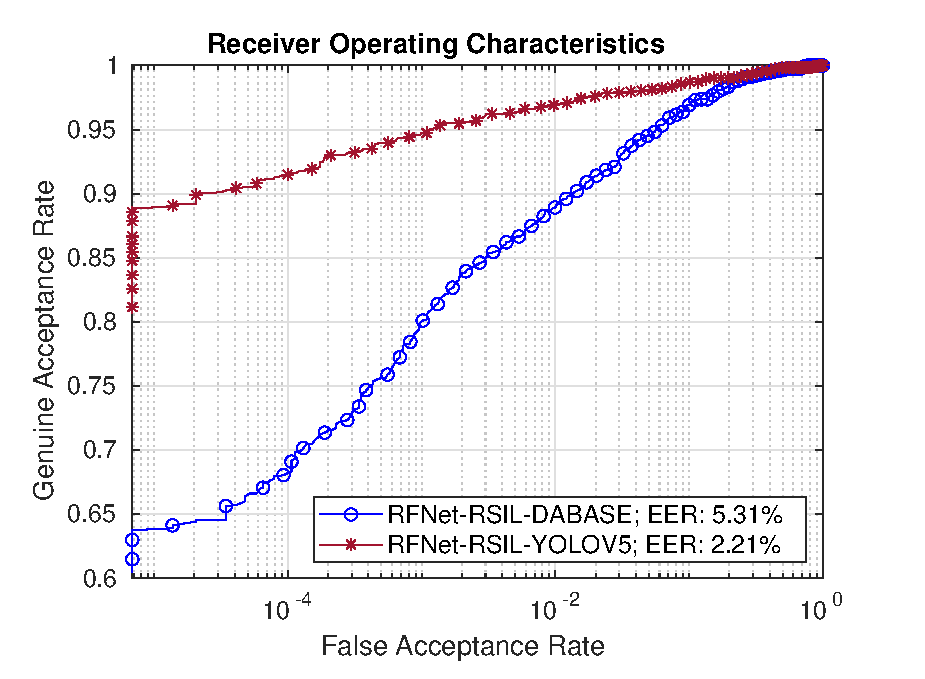
\includegraphics[width=\linewidth]{Figures/yolov5vsdatabase/fkv3-roc_compare_new.eps}
	\end{subfigure}
	\begin{subfigure}[b]{0.45\linewidth}
		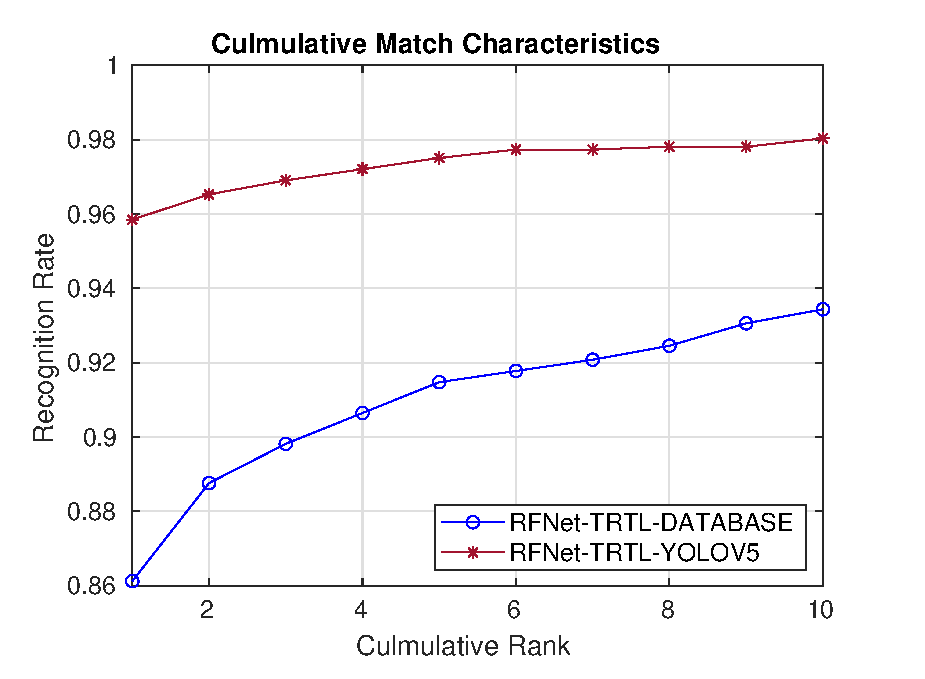
\includegraphics[width=\linewidth]{Figures/yolov5vsdatabase/fkv3-cmc_compare_new.eps}
	\end{subfigure}
	\caption{Compare performance on the Finger Knuckle V3 Dataset (with deformable)}
\end{figure}

\begin{figure}[H]
	\centering
	\begin{subfigure}[b]{0.45\linewidth}
		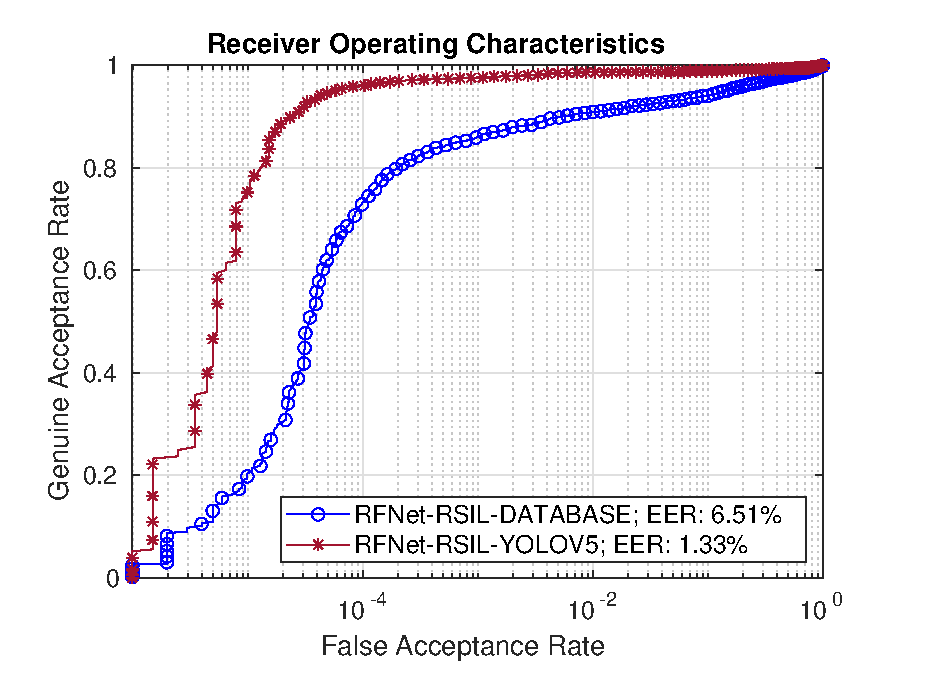
\includegraphics[width=\linewidth]{Figures/yolov5vsdatabase/hd-roc_compare_new.eps}
	\end{subfigure}
	\begin{subfigure}[b]{0.45\linewidth}
		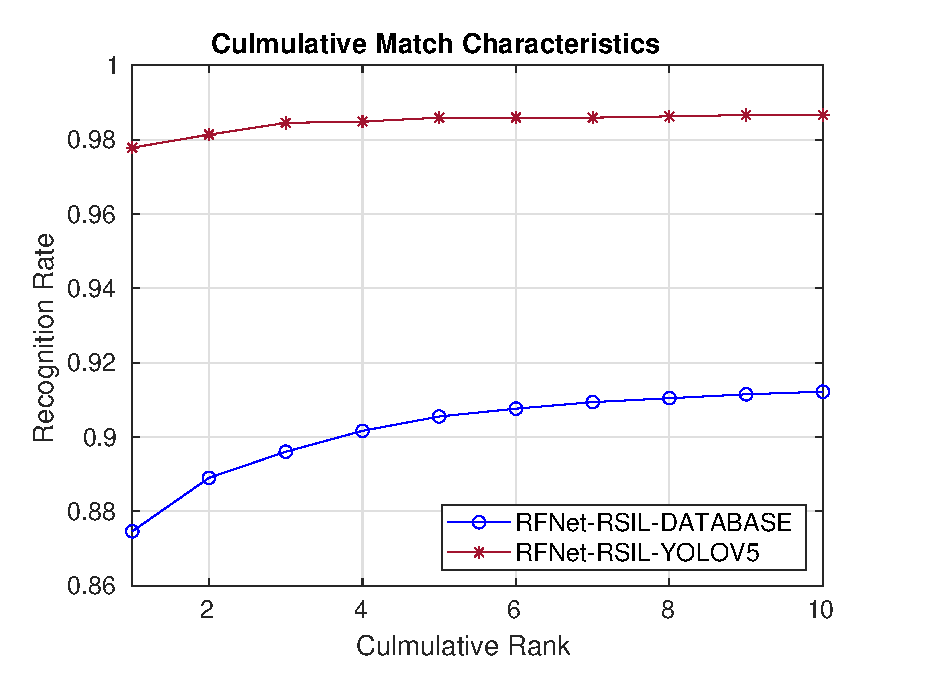
\includegraphics[width=\linewidth]{Figures/yolov5vsdatabase/hd-cmc_compare_new.eps}
	\end{subfigure}
	\caption{Compare performance on the Index Finger of the Hand Dorsal Image Database.}
\end{figure}

From the above figures, we can clearly get the conclusion that quality of segmented finger knuckle of YOLOv5 is better than the segmented finger knuckle of dataset through the ROC curve and CMC curve. Especially on the Hand Dorsal Image Database, the EER value can drop from $6.51\%$ to $1.33\%$. 



 \subsection{Online Contactless Finger Knuckle Identification Performance}

 For proving our contactless and online finger knuckle identification performance, we capture  52 subjects and each subject can offer about 15-20s contactless finger knuckle video. The minimum frame rate of the videos we offer is 30 frames per second. We choose two method to get the contactless finger knuckle images, one is that we get 1 image per second, another one is that we get 6 images per second for testing online matching performance. Because the shortest video is 15s, for 1 image per second, we can totally get $52*15 = 780$ finger knuckle images for keeping the same number of samples result in $52*15 =1789 $ genuine matching scores and $52*51*15 = 39780$ imposter matching scores. In terms of the 6 images per second, we can get $52*15*6=4680$ finger knuckle samples, result in $52*90=4680$ genuine matching scores and $52*51*90=238680$ imposter matching scores.
 .............

 \begin{figure}[H]
	\centering
	\begin{subfigure}[b]{0.45\linewidth}
		\includegraphics[width=\linewidth]{Figures/online-performance/1s1f-roc_compare_new.eps}
		\caption{}
	\end{subfigure}
	\begin{subfigure}[b]{0.45\linewidth}
		\includegraphics[width=\linewidth]{Figures/online-performance/1s1f-cmc_compare_new.eps}
		\caption{}
	\end{subfigure}
	\caption{Comparative ROC (a) and corresponding CMC (b) with one session protocol for }
\end{figure}

\begin{figure}[H]
	\centering
	\begin{subfigure}[b]{0.45\linewidth}
		\includegraphics[width=\linewidth]{Figures/online-performance/1s6f-roc_compare_new.eps}
	\end{subfigure}
	\begin{subfigure}[b]{0.45\linewidth}
		\includegraphics[width=\linewidth]{Figures/online-performance/1s6f-cmc_compare_new.eps}
	\end{subfigure}
	\caption{}
\end{figure}
\input{references.tex}

\end{document}
